\documentclass[twocolumn]{summery_4.0}
\title{Experimentalphysik IV - Zusammenfassung}

\begin{document}
\maketitle
\tableofcontents

\section{Einführung in die atomare Welt}
\subsection{Erste Einweise auf eine Diskretisierung auf der kleinsten Ebene}
\begin{itemize}
    \item[Gesetz der konstanten Proportionen:] In der Chemie wurde im 19. Jahrhundert entdeckt, dass viele chemische Reaktionen in ganzzahligen Verhältnissen ablaufen, z.B. für 100g Wasser: 11.1g Wasserstoff + 88.9g Sauerstoff $\to$ Massenverhältnis 1:8 
    \item[Gesetz konstanter Volumina:] Bei gleicher Temperatur und Druck reagieren Gase in konstanten ganzzahligen Volumenverhältnissen. Dies kann mit der idealen Gasgleichung so erklärt werden, dass bei gleicher Temperatur und Druck das  Volumenverhältnissen gleich dem Verhältnis an Teilchenzahlen ist $\frac{V_1}{V_2} = \frac{N_1}{N_2}$.
    \item[Periodizität chemischer Eigenschaften von Elementen mit Ordnungszahl $Z$:] Mitte des 19ten Jahrhunderts durch Dmitri Mendelejew und Lothar
    Meyer entdeckt; Führte zur Entwicklung des Periodensystems.
    \item[Brownsche Molekularbewegung:] Zitterbewegungen kleiner Mikropartikel aufgrund von zufälligen Kollisionen mit Atomen/Molekülen in der Umgebung.
\end{itemize}

\subsection{Röntgenbeugung}

\subsection{Experimente}
\subsection{Massenspektrometer nach Thomsons (1912)}
\begin{figure}[H]
    \centering
    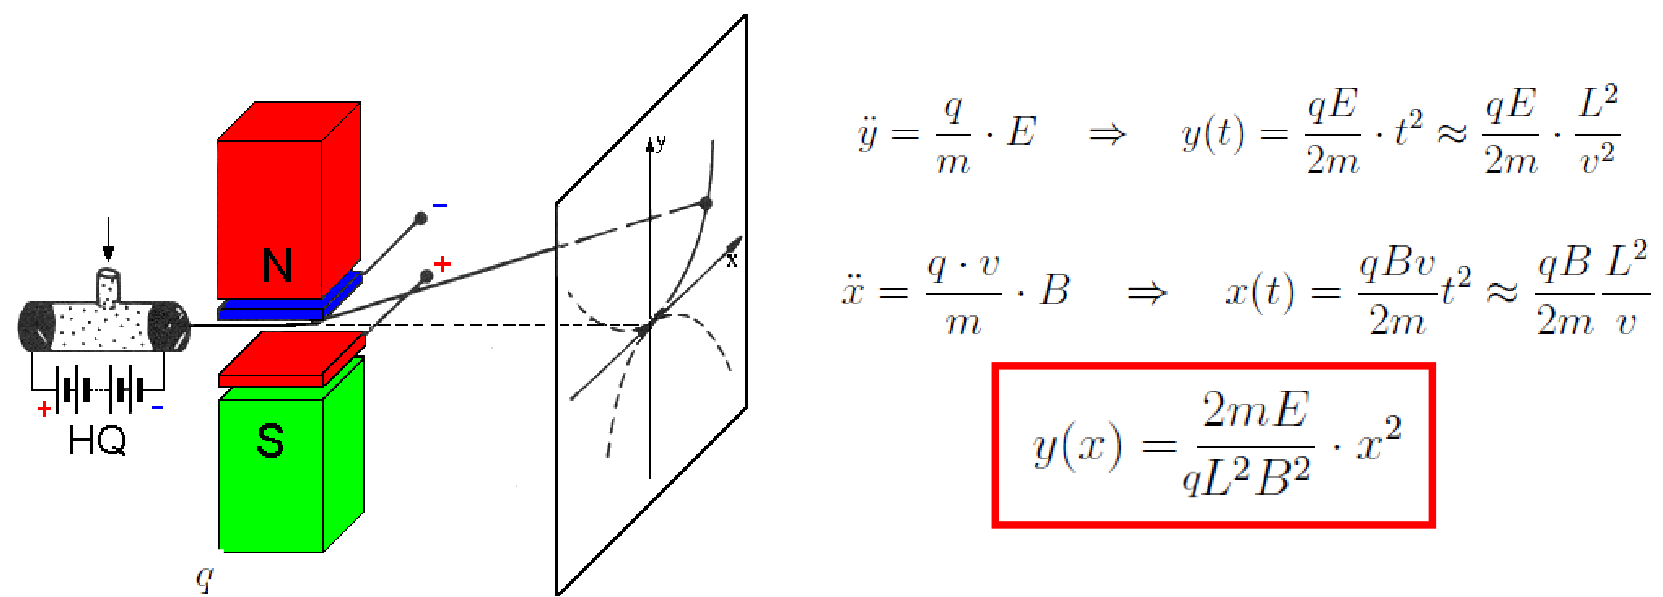
\includegraphics[width=0.7\textwidth]{massenspektrometer_nach_thomson.png}
\end{figure}
Alle Atome gleicher Masse und Ladung landen auf der gleichen Parabel, sie relative natürliche Häufgkeit einzelner Isotope kann aus der Stärke der Schwärzung im Bild eines Massenspektrometers ermittelt werden.

\subsection{Schrödinger-Gleichung}
\begin{align*}
    E\Psi &= H\Psi = \hug{-\frac{\hbar^2\Delta}{2m}+V} 
\end{align*}
\subsubsection{Tunnelwahrscheinlichkeit}
\begin{align*}
    P\sub{Tunnel} = \frac{16E}{V_0^2}(V_0-E) e^{-\frac{2a}{\hbar} \sqrt{2m(V_0 -E)}}\note a \equiv \te{Breite der Barriere}
\end{align*}


\end{document}